%
% Uvod
%

\chapter{Úvod}

Každý linuxový server alebo osobný počítač môže slúžiť na niečo iné. Preto je
veľmi náročné vytvoriť linuxovú distribúciu, ktorá by pokrývala požiadavky
každého a~bola optimalizovaná pre všetky operácie. Preto je potrebné systém
nastaviť tak, aby presne vyhovoval naším potrebám a~získali sme maximálny výkon
pre naše potreby. Kedže sa jedná a~množstvo druhov nastavení, vznikol balíček
\emph{tuned}\cite{tunedHomepage}, ktorý ich zahrňuje.

Cieľom tejto práce je priblížiť \emph{tuned}, zhrnúť jeho hlavné funkcie,
popísať profily a~na záver implementovať sadu testov pre I/O operácie nad
najpoužívanejšími súborovými systémami a~diskovými zariadeniami. Na záver budú
testy spustené a~výsledky vyhodnotené.

%
% Popis komponenty
%

\chapter{Popis komponenty tuned}

Balíček \emph{tuned} je primárne napísaný pre linuxovú distribúciu
Fedora\cite{fedoraHomepage} a~Red Hat Enterprise Linux. Démon \emph{tuned} neustále
beží, skenuje systém a~upravuje nastavenia podľa potreby. Napríklad najväčšia
záťaž na disk je pri štarte systému alebo pri ukladaní dát na disk (napríklad
filmov). Inak je disk skoro nečinný. \emph{tuned} dokáže optimalizovať zápis práve v
tej dobe, keď je to potreba. Rovnako je to aj pri sieťových operáciach.

Súčasťou \emph{tuned} je aj program \emph{tuned-adm}, ktorý nám dovoľuje
prepínať medzi profilmi. Každý z~profilov slúži na iné zameranie a~napriamo
podľa toho upravuje systém, čím dosahujeme ešte lepšie výsledky.

%
% Historia tuned
%

\subsection{História \emph{tuned}}
\label{sec:historiaTuned}

%TODO: Skontrolovat rok
Komponenta \emph{tuned} je vyvýjaná od roku 2008. Prvými autormi boli
\emph{Philip Knirsh} a~\emph{Thomas WoVerner}. Dnes sú najväčšími
prispievatelia \emph{Ján Včelák}, \emph{Jaroslav Škarvada} a~\emph{Ján Kaluža}.
Dnes je \emph{tuned} vo verzii \emph{2}. Medzi verziou \emph{1} a~\emph{2} je
veľký rozdiel, pretože bol celý kód od základov prepísaný. Jedna z~najväčších
zmien je v~používaní \emph{D-BUS} \footnote{Systém pre jednoduché zasielanie
správ a~komunikáciu medzi aplikáciami}. Ďalšia zmena je v~profiloch. Niektoré
profily boli zmenené alebo odobraté. Pre zachovanie spätnej kompatibility
vznikol preto balík \emph{tuned-profiles-compat}, ktorý obsahuje všetky profily
z verzie \emph{tuned 1}.

%
% Profily tuned
%

\section{Profily}

Profily su hlavne zamerané na CPU, disky, sieť a~FSB \footnote{Front-Side Bus -
datová zbernica, ktorá zaisťuje komunikáciu medzi CPU a~hardvérom. Využíva sa v
procesoroch \emph{Intel}}. Samotný balíček obsahuje niekoľko predvolených
profilov a~ako základný profil je po spustení \emph{tuned} profil \emph{balanced}.

Profily si môžeme aj samy vytvárať. Ak si nie sme istý, čo je potrebné upraviť,
môžeme využiť odporúčania z~programu \emph{powertop}\cite{powertopHomepage}~a
za pomoci skriptu \emph{powertop2tuned} si nechať profil vytvoriť automaticky
na základe výstupu z~\emph{powertop}. Bližšiemu popisu profilov sa venuje
sekcia \ref{sec:prehladProfilov}. 


%
% Prehlad profilov
%

\subsection{Prehľad profilov}
\label{sec:prehladProfilov}

Profily \emph{tuned} sa nachádzajú v~adresári \emph{/usr/lib/tuned}. V~tomto
adresári sa taktiež nachádza súbor s~funkciami, ktoré tieto profily využívajú.
Práve tieto súbory sú najviac vyvýjané a~menené.

Prehľad profilov zo základného balíčka \emph{tuned}. Zoznam je platný pre
verziu \texttt{tuned-2.2.2-1} na \emph{Fedora 18}:

\begin{itemize}
    \item \textbf{balanced} - predvolený profil pre väčšinu systémov s~výnimkou virtuálnych
    \item \textbf{latency-performance} - %TODO
    \item \textbf{powersave} - na zníženie odberu
    \item \textbf{throughput-performance}i %TODO
    \item \textbf{virtual-guest} - predvolený profil pre virtuálne systémy
    \item \textbf{virtual-host} %TODO
\end{itemize}

Balíček \emph{tuned-profiles-compat} rozširuje zoznam o~tieto ďalšie profily:

\begin{itemize}
    \item \textbf{default}
    \item \textbf{desktop-powersave}
    \item \textbf{enterprise-storage}
    \item \textbf{laptop-ac-powersave}
    \item \textbf{laptop-battery-powersave}
    \item \textbf{server-powersave}
    \item \textbf{spindown-disk}
\end{itemize}

Medzi najčastejšie operácie profilov patrí menenie governoru\footnote{Rýchlosť
procesora je možné meniť a~tým šetriť energiu v čase, ked ho naplno
nevyužívame. Túto rýchlosť ovplyvňujú rôzne druhy plánovačov.} procesoru medzi
\texttt{ondeman}|\footnote{Nastavuje rýchlosť procesora podľa využitia.}
a~\texttt{performance}\footnote{Nastaví rýchlosť procesora na najvyššiu hodnotu
bez ohľadu na využitie.}. Viac o~tejto vlastnosti je možné dočítať sa na wiki
stránkach Arch Linuxu\cite{arch:governor}.

Ďalej je to nastavovanie plánovačov diskov. Toto nastavenie sa mení v~súbore
\texttt{/sys\-/block\-/<dev>\-/queue\-/scheduler}. Niektoré profily ho prepínajú z
predvoleného plánovača na \emph{deadline}\footnote{Tento plánovač sa používa
pre zníženie latencie. Obsahuje dve fronty a~každá požiadavka má deadline}.
Viac o~plánovačoch diskov je možné sa dočítať na stránkach dokumentácie
\emph{OpenSuse}\cite{suse:scheduler} alebo v článku \cite{book:scheduler}.

Niektoré profily taktiež vypínajú bariéry\footnote{Vypnutím bariér hrozí
poškodenie dát pri odpojení napájania diskov, pokiaľ disk nemá záložnú
batériu.} pri pripojovaní diskov. 

%
% Plan testovania
%

\chapter{Plán testovania pre Fedora Linux}

\section{Test Plan Identifier}
\section{References}

%\section{Introduction}
\section{Úvod}

Na testovanie tuned využijeme pomocnú knižnicu beakerlib
\cite{beakerlibHomepage} pre jednoduchšie písanie testov a~prehľadnejšiu
interpretáciu dosiahnutých výsledkov. Cieľom testov je analýza, či tuned
profily spĺňajú požadované vlastnosti.

%\section{Test Items}
\section{Testovacie položky}

Napísané testy budú overovať správnu funkcionalitu tuned démona a~taktiež
ktune profilov v~zameraní na CPU, disky a~sieťové operácie. Všetky testy budú
pripravené pre linuxovú distribúciu Fedora 17 \cite{fedoraHomepage}.

%\section{Software Risk Issues}
\section{Softvérové riziká}

V prípade zlyhania niektorých testov môže prísť k~poškodeniu už pripojených
diskov alebo k~rozladeniu sieťových rozhraní. Preto je vhodné spúšťat sadu
testov na virtuálnom stroji. V~prípade vydania novej verzie tuned alebo inej
použitej komponenty je tu riziko, že testy nebudú stabilné a~môžu sa správať
nepredvídateľne.

%\section{Features to be Tested}
\section{Čo sa bude testovať}

Hostiteľský systém bude spúšťať predpripravené obrazy virtualizovaného systému
Fedora 17. K~virtualizovanému systému bude pripájať ďalšie disky. Tieto nové
disky budú formátované na najpoužívanejšie súborové systémy a~testované ich
rýchlosti pri rôznych profiloch tuned.

Na testovacie účely použijeme najnovšiu verziu tuned z~repozitára.

%\section{Features not to be Tested}
\section{Čo sa nebude testovať}

Pretože testy bežia na virtualizovanom hardvéri, nie všetko je možné otestovať.
Napríklad virtuálny procesor nepodporuje Cx stavy \footnote{Cx sú stavy, v
ktorých sa môže vyskytovať procesor, typicky firmy Intel. Tieto stavy sa volajú
Spiacie stavy (ang. Sleep states) \cite{sleepStates}. Spiace stavy procesoru
slúžia na šetrenie energie.}, ktoré ovplyvňuje profil \emph{latency-performance} a
preto nie je možné spoľahlivo a~automatizovane otestovať ich správu.

\section{Approach}

%\section{Item Pass/Fail Criteria}
\section{Kritéria pre splnenie testov}

Počas testovania so zapnutým démonom tuned by všetky I/O operácie diskov mali
byť rýchlejšie alebo aspoň tak rýchle ako s~vypnutým tuned.

\section{Suspension Criteria and Resumption Requirements}
\section{Test Deliverables}
\section{Remaining Test Tasks}
\section{Environmental Needs}
\section{Staffing and Training Needs}
\section{Responsibilities}
\section{Schedule}
\section{Planning Risks and Contingencies}
\section{Approvals}
\section{Glossary}

%
% Testovanie
%

\chapter{Testovanie}

\section{Príprava systému}

Pred testovaním je potrebné pripraviť si nainštalovaný systém Fedora 17 ako
obraz disku. Tento obraz sa bude spúšťať cez qemu-kvm. Disk, na ktorom sa bude
testovať rýchlosť zápisu a čítania by mal byť v~ideálnom prípade nekešovaný.
Pred testovaním aj po testovaním je potrebné hostiteľský aj virtualizovaný
systém synchronizovať aj zmazať aj nakešované stránky (Algoritmus
\ref{alg:sync}).

\begin{algorithm}
    \label{alg:sync}
    \caption{Synchronizácia systému}
    /bin/sync\\
    echo 3 \textgreater /proc/sys/vm/drop\_caches
\end{algorithm}

Každé miesto, kde je možnosť, že by systém si uchovával nejaké nakešované data,
ktoré by mohli ovplyvniť výsledky testovania je potrebné poznať (Obrázok \ref{graf-cache}).

\begin{figure}[ht]
\begin{center}
  \makebox[\textwidth]{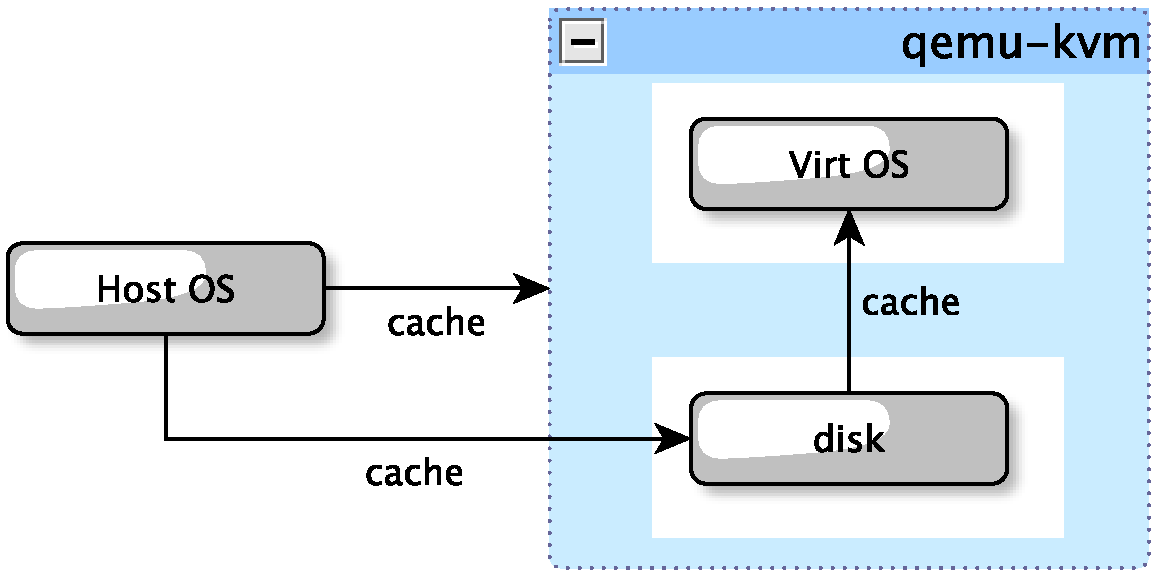
\includegraphics[width=\paperwidth/2]{data/cache.pdf}}
  \caption{Vyznačenie miest, kde môže nastať kešovanie}
  \label{graf-cache}
\end{center}
\end{figure}

Virtualizovaný systém musí obsahovať všetky potrebné balíčky, ktorých programy
sa používajú v~testoch. Spúštanie testov bude prebiehať cez ssh spojenie a
preto je potrebné si zabezpečiť bezchybnú komunikáciu medzi hostiteľským a
virtualizovaným systémom - ideálne certifikát bez hesla pre root užívateľa a
statickú IP adresu, ktorá sa nezmení po reštarte systému.

\section{Použitie virtuálneho stroja}

Testovanie diskových operácií prebieha vo virtuálnom stroji za použitia \emph{qemu-kvm} pod \emph{libvirtd}. 

\chapter{Záver}
Zaver

